\documentclass[11pt]{article}
\usepackage[T1]{fontenc}
\usepackage[utf8]{inputenc}
\usepackage{lmodern}
\usepackage[a4paper,margin=1in]{geometry}
\usepackage{amsmath,amssymb,amsthm,amscd,mathtools}
\usepackage{microtype}
\usepackage{tikz}
\usetikzlibrary{arrows.meta,decorations.markings}
\PassOptionsToPackage{hyphens}{url}
\usepackage[hidelinks]{hyperref}
\hypersetup{pdftitle={The p-adic section conjecture},pdfauthor={OpenAI}}
\usepackage{enumitem}
\numberwithin{equation}{section}
\newtheorem{theorem}{Theorem}[section]
\newtheorem{proposition}[theorem]{Proposition}
\newtheorem{lemma}[theorem]{Lemma}
\newtheorem{corollary}[theorem]{Corollary}
\theoremstyle{remark}
\newtheorem{remark}[theorem]{Remark}
\newtheorem{definition}[theorem]{Definition}
\DeclareMathOperator{\Gal}{Gal}
\title{The p-adic section conjecture}
\author{OpenAI}
\date{September 24, 2026}
\pdfinfoomitdate=1
\pdftrailerid{}
\pdfsuppressptexinfo=15
\begin{document}
\maketitle
\begin{abstract}
We prove the local $p$-adic section conjecture for smooth proper
geometrically connected curves of genus at least two, over every finite
extension of $\mathbb Q_p$.
Combined with established finite-descent theorems, this also yields the
global section conjecture for smooth proper geometrically connected
curves of genus at least two over number fields when their finite-cover
descent locus equals their rational points; this includes $X_0(N)$ and
$X_1(N)$ of genus at least two over $\mathbb Q$.
\end{abstract}
\tableofcontents
\section{Introduction}\label{sec:introduction}

Let $p$ be a prime, let $k/\mathbb Q_p$ be a finite extension, and let
$X/k$ be a smooth proper geometrically connected curve of genus at least
two. Choose an algebraic closure $\bar k$ and a geometric base point
of $X$. The full arithmetic \'etale fundamental group fits into
\begin{equation}\label{eq:fundamental-sequence}
 1\longrightarrow\Delta_X\longrightarrow\Pi_X
   \longrightarrow G_k\longrightarrow1,
 \qquad
 \Delta_X=\pi_1(X_{\bar k}),\quad \Pi_X=\pi_1(X),\quad
 G_k=\Gal(\bar k/k).
\end{equation}
A rational point $a\in X(k)$ induces a continuous group-homomorphic
section $s_a:G_k\to\Pi_X$. Its class under conjugation by $\Delta_X$
is independent of the path used to identify base points. The local
$p$-adic section conjecture asserts that this construction accounts for
all sections, and distinguishes all rational points.

A section whose class comes from a rational point is called
\emph{geometric}. The conjecture thus asks whether rational points can
be recovered from the splittings of the arithmetic fundamental group.
It is a local analogue of the section conjecture in Grothendieck's
letter to Faltings of 27 June 1983, formulated over fields finitely
generated over the prime field
\cite[equation~(7) and the subsequent properness correction]{GrothendieckLetter}.
The local question retains the full arithmetic and geometric groups
in~\eqref{eq:fundamental-sequence}, while bringing the geometry of
$p$-adic valuations and reduction into the problem.

\begin{theorem}\label{thm:section}
For every prime $p$, every finite extension $k/\mathbb Q_p$, and every
smooth proper geometrically connected curve $X/k$ of genus at least two,
the map
\[
 X(k)\longrightarrow
 \left\{\begin{gathered}
 s:G_k\to\pi_1(X)\text{ a continuous group homomorphism}\\
 \text{such that }(\pi_1(X)\to G_k)\circ s=\mathrm{id}_{G_k}
 \end{gathered}\right\}\big/\pi_1(X_{\bar k})
\]
is bijective. The quotient is by conjugation by the full geometric
\'etale fundamental group.
\end{theorem}

\subsection{Earlier results and the lifting problem}

The birational analogue replaces the arithmetic \'etale fundamental
group by the absolute Galois group of the curve's function field.
For a Galois extension with a chosen valuation, the
\emph{decomposition group} consists of the automorphisms preserving
its valuation ring.
Koenigsmann proves that every birational section over a finite extension
of $\mathbb Q_p$ is contained in the decomposition group of a rational
point \cite[preprint version, Proposition~2.4(2)]{Koenigsmann}.
Pop subsequently obtains a birational criterion from sections of an
elementary abelian quotient that lift to the corresponding elementary
metabelian quotient
\cite[Theorems~A and~A$'$]{PopBirational}.
These results make the passage from an \'etale section to a birational
section a natural objective. Such a lift is additional information:
a section of the quotient group in~\eqref{eq:fundamental-sequence} does
not by itself supply a splitting of the absolute Galois sequence.

Pop--Stix localize every \'etale section at a valuation extending the
$p$-adic valuation \cite[preprint version, Theorem~26]{PopStix}.
This reduces the problem to understanding which valuations can support
a section. Pajwani develops this valuative approach through \'etale
homotopy and fixed points in Berkovich spaces
\cite[preprint version, Theorem~1.4 and Corollary~1.5]{Pajwani}.
The passage from a fixed valuation to a rational point remains the
geometric issue addressed here.

Recent results also constrain the possible nongeometric sections.
Bresciani introduces toric sections and proves the section conjecture
for them; they map
injectively to the set of \'etale sections
\cite[Definition~3.7 and Theorems~1.4 and~5.10]{BrescianiToric}.
For an arbitrary nongeometric \'etale section, his Theorem~1.5 produces
a finite \'etale neighbourhood whose index is divisible by $p$.
Here a neighbourhood is a connected finite \'etale cover to which the
section lifts, and the index of a curve is the greatest common divisor
of the degrees of its closed points.
In a different direction, Betts--Stix prove finiteness of the local
image of global Selmer sections for smooth proper geometrically
connected curves of genus at least two over number fields containing no CM subfield
\cite[preprint version, Theorem~A]{BettsStix}.
Their Selmer sections already arise from points at every completion;
the finiteness assertion concerns the local images of this globally
constrained set of sections.

Our lifting step is a statement about completions of the universal
\'etale function field. It compares the absolute and \'etale
decomposition groups at every rank-one valuation extending the
$p$-adic norm. This supplies the birational lift at precisely the
valuations that must be excluded from the Pop--Stix localization.

\subsection{The completion statement}

Put $K=k(X)$ and choose a separable closure $K^{\mathrm{sep}}$ containing
$\bar k$. Let $\widetilde K\subset K^{\mathrm{sep}}$ be the compositum
of the function fields of all connected finite \'etale covers of $X$,
with all their $K$-embeddings in $K^{\mathrm{sep}}$. Then
$\Gal(\widetilde K/K)=\Pi_X$ after the chosen base point identification.
A real-valued rank-one norm on $K$ means a nonarchimedean field absolute
value with values in $\mathbb R_{\ge0}$; in particular its support is
zero. We normalize an extension of the $p$-adic norm by $|p|=p^{-1}$.

\begin{theorem}\label{thm:completion}
Let $p$ be a prime, let $k/\mathbb Q_p$ be finite, and let $X/k$ be a
smooth proper geometrically connected curve of genus at least two.
Put $K=k(X)$, choose a separable closure $K^{\mathrm{sep}}$, and let
$\widetilde K\subset K^{\mathrm{sep}}$ be the compositum of the function
fields of all connected finite \'etale covers of $X$, with all their
$K$-embeddings.
For every real-valued rank-one norm on $K$ extending the normalized
$p$-adic norm on $k$, and every prolongation to $K^{\mathrm{sep}}$, set
\[
 E=\widehat{K^{\mathrm{sep}}},\qquad
 H=\widehat{\widetilde K}\subset E,
\]
where the completions use that fixed prolongation.
Then the specified subfield $K^{\mathrm{sep}}$ of $E$ is contained in $H$.
\end{theorem}

The statement concerns the chosen copies of these fields inside one
completion. Write $D_\nu(L/K)$ for the decomposition group of a
valuation $\nu$ on a Galois extension $L/K$.
Corollary~\ref{cor:decomposition} uses Theorem~\ref{thm:completion} to
identify the decomposition group in $K^{\mathrm{sep}}/K$ with the one
in $\widetilde K/K$. Indeed, an automorphism in the kernel fixes a
dense subfield of $H$ and hence fixes $K^{\mathrm{sep}}$.

A section localized at a rank-one valuation therefore lifts to a
birational section. Koenigsmann's theorem places this lifted section
also at a rational point. Its fixed field would then carry two
inequivalent henselian rank-one valuations, one extending the $p$-adic
valuation and the other trivial on constants. The contradiction is an
explicit instance of the classical two-valuation principle associated
with F.~K.~Schmidt \cite{SchmidtValuations}; Section~\ref{sec:sections}
gives the needed approximation and square-root argument, including
$p=2$.

Rank-two valuations are handled by their rank-one coarsenings. The
remaining case is a closed-point valuation refined by the $p$-adic
valuation on its residue field, called type~$2h$ by Pop--Stix.
The surjection of the section onto $G_k$ forces that closed point to
be rational, and their type-$2h$ analysis then identifies the section
\cite[preprint version, Section~6.1]{PopStix}.
Section~\ref{sec:sections} completes this argument and proves
injectivity of the point-to-section map by Kummer theory on the
Jacobian.

\subsection{Two stages of collar roots}

The geometric content lies in Theorem~\ref{thm:completion}.
A finite extension of $\bar k(X)$ is the function field of a finite
curve cover, which may have branch points. Near such a point, with
local coordinate $t$, a branch has the form $t=z^e$.
If another cover supplies a root of $t$ of order divisible by all
these branch indices, the pulled-back cover splits over an annulus
around the branch point. One can then replace the part over the inner
disk by a trivial cover and glue to obtain an \'etale cover.
The roots must exist on the \emph{entire} inverse image of the annulus:
a root on only one sheet does not trivialize the full cover needed
for gluing. We use this operation twice, with different sources of
collar roots.

This gluing and algebraization method belongs to the formal and rigid
analytic patching tradition of Harbater and Liu
\cite{HarbaterPatching,LiuPatching}. Poineau treats the corresponding
Berkovich framework \cite[Section~1 and Appendix~A]{GAGA}.
Section~\ref{sec:patching} proves the precise replacement and
field-embedding statements used here. In particular, evaluating the
resulting exterior analytic map retains the specified valued field
embedding; the map itself need not descend to $\bar k$.

Fix an odd prime $\ell\ne p$. In the first stage, coordinates on the
node annuli of a stable model acquire $\ell$-th roots on suitable
finite \'etale covers. The construction uses the lifting theorem of
Amini--Baker--Brugall\'e--Rabinoff, which realizes tame coverings of
metrized complexes as curve covers \cite[Theorem~7.7]{ABBR}.
A metrized complex records the skeleton together with the residue
curve at each vertex and the marked points corresponding to edge ends.
Small collars around arbitrary branch points need not themselves be
stable node annuli. The resolution of nonsingularities theorem of
Mochizuki--Tsujimura supplies a finite \'etale cover whose stable model
maps to a prescribed semistable model
\cite[Theorem~A and Proposition~2.4(iv)]{MochizukiTsujimura}.
This extends Tamagawa's result for closed points on a stable model
\cite[Theorem~0.2(v)]{TamagawaRNS} and Lepage's corresponding resolution
theorem for Mumford curves \cite[Theorem~2.7]{LepageRNS}.
The general theorem of Mochizuki--Tsujimura allows us to move these
collars into the stable-node construction.
Patching then places in $H$ every finite Galois extension whose
horizontal ramification indices divide $\ell$. Here horizontal
indices refer to ramification at closed points over $\bar k$.
Section~\ref{sec:tame-roots} proves this first stage.

The second stage produces roots of arbitrary positive order $m$ while
keeping the auxiliary cover's horizontal indices dividing
$\ell$. We construct a cyclic cover of the projective line whose
skeleton has two vertices and $\ell$ parallel edges. A cycle using
two distinct edges gives a character of the torus uniformizing its
Jacobian. Along a chosen annulus that character has slope one, so it
is a constant times the annular coordinate times an analytic unit
close to one. Figure~\ref{fig:parallel-edges} shows the geometry.
This uses the nonarchimedean uniformization theory of Raynaud and
Bosch--L\"utkebohmert \cite{RaynaudUniformization,BoschLutkebohmert}
and the compatibility of classical and tropical Abel--Jacobi maps
proved by Baker--Rabinoff
\cite[Proposition~6.1 and Corollary~6.6]{BakerRabinoff}.

Pullback by multiplication by $m$ on the Jacobian supplies a root of
the character on the whole inverse annulus. On a sufficiently long
middle collar, the remaining unit has an $m$-th root by the $p$-adic
logarithm and exponential. This yields a root of the coordinate itself.
The auxiliary covers still have horizontal indices dividing $\ell$,
so the first stage places their function fields in $H$.
Section~\ref{sec:arbitrary-roots} constructs these roots, and a second
application of patching in Section~\ref{sec:realization} realizes
arbitrary finite Galois extensions in the same completion.
The common requirement of roots on every inverse-image sheet is what
allows both stages to use the same patching proposition.

\subsection{Global consequences}

The local theorem also identifies the possible localizations of global
sections. Let $C/F$ be a smooth proper geometrically connected curve of
genus at least two over a number field. A global section determines a
point of $C(F_v)$ at every finite place by Theorem~\ref{thm:section},
and a connected component of $C(F_v)$ at every real place by the real
section theorem \cite[Introduction, Theorem]{BrescianiVistoliReal}.
Together these form a \emph{modified adelic point}; complex places
contribute no factor. The finite-cover descent locus consists of the
tuples that lift to some global twist of each torsor under a finite
$F$-group scheme. Proposition~\ref{prop:localization-image} shows that
this locus is exactly the image of global sections under localization.
Both inclusions use the descent bridge of Harari--Stix
\cite[preprint version, Theorem~2.1 and Remark~2.2(1)]{HarariStixFiniteDescent}.

When this finite-cover locus consists exactly of the diagonal rational
points, Stix's finite-support theorem identifies every global section
with a point section
\cite[arXiv version, Corollary~5]{StixFiniteSupport}.
The resulting bijection is Theorem~\ref{thm:global-descent}.
Stoll's finite-descent criteria supply the required equality when the
curve has a nonconstant morphism over its number field to an abelian
variety with finitely many rational points and trivial divisible
Tate--Shafarevich subgroup, or when its Jacobian has these properties.
They also cover the smooth projective modular curves $X_0(N)$ and
$X_1(N)$ of genus at least two over $\mathbb Q$
\cite[Corollary~8.1, Theorem~8.6, and Corollary~8.8]{StollFiniteDescent},
with the corrections in \cite{StollFiniteDescentErrata}.
The Selmer converse in the companion article
\cite[Theorem~1.1]{OpenAISelmerConverse2026} gives a further arithmetic
test for an elliptic target over $\mathbb Q$: vanishing of its full
$p$-power Selmer corank at one prime.
Section~\ref{sec:global-sections} states the precise hypotheses and
deductions for these cases.

The localization description also yields constraints without assuming
that the finite-cover locus consists of rational points. Every ordinary
adelic representative of a localization tuple survives linear descent
and lies in the Brauer--Manin set, by further results of Harari--Stix
\cite[preprint version, Corollary~3.1 and Theorem~4.1]{HarariStixFiniteDescent}.
If $F$ contains no CM subfield, Betts--Stix's theorem makes the projection
of the localization image to $C(F_v)$ finite at every finite place $v$
\cite[preprint version, Theorem~A]{BettsStix}.
These statements constrain the localization image; the finite-cover
equality remains a separate arithmetic hypothesis in the global
section-conjecture criterion.

\section{Fields, analytic points, and horizontal ramification}
\label{sec:preliminaries}

Fix the data and the prolonged norm of Theorem~\ref{thm:completion}.
All subsequent field inclusions refer to these choices. We have
\[
 K\subset K_0:=\bar k(X)\subset\widetilde K\subset K^{\mathrm{sep}}
 \subset E,
 \qquad H=\widehat{\widetilde K}\subset E.
\]
The inclusion of the completion $H$ into $E$ is isometric: it identifies
$H$ with the closure of $\widetilde K$ in $E$. Since $k$ is complete, the
restriction of the chosen norm to $\bar k$ is its unique prolongation.
Thus $\Omega:=\widehat{\bar k}$ is a specified subfield of $H$.
It is algebraically closed and has additive value group $\mathbb Q$,
with the normalization $v=-\log_p|\cdot|$. The equality of value groups
before and after completion follows because every nonzero limit has
the same norm as sufficiently close approximants.

We use Berkovich analytifications over $\Omega$. A field embedding
$K_0\hookrightarrow H$ determines a point of $X_{\bar k}(H)$ supported
at the generic point of $X_{\bar k}$. Together with the specified
embedding $\Omega\hookrightarrow H$, it determines a point of
$X_\Omega(H)$, whose analytic image we denote by $\xi$. Its projection
to $X_{\bar k}$ is generic; its support on $X_\Omega$ need not be
generic. In particular, $\xi$ can be an $\Omega$-rational point.
We retain the whole $H$-valued point, including the embedding of its
completed residue field into $H$, whenever we use $\xi$.

If $F/K_0$ is finite, its normalization gives a smooth proper connected
curve over $\bar k$ with a finite map to $X_{\bar k}$. We call the
ramification indices of this map at closed points \emph{horizontal
ramification indices}. The corresponding discrete valuations are trivial
on $\bar k$ and have residue characteristic zero. These indices are
unrelated to possible wild ramification on a characteristic-$p$
reduction model.

Fix an odd prime $\ell\ne p$. Inside $K^{\mathrm{sep}}$, let $L_\ell$
be the compositum of all finite Galois extensions $F/K_0$ whose horizontal
ramification indices divide $\ell$. The unramified extensions are
included. In particular $\widetilde K\subset L_\ell$: the universal
\'etale field over $K_0$ is the same field $\widetilde K$ after constants
are included. One may see this by descending any finite \'etale cover of
$X_{\bar k}$ to a finite extension of $k$ and then composing with the
finite \'etale constant-field cover of $X$.

The field-theoretic goal can be displayed as follows. The top row consists
of the defining inclusions; the two right vertical arrows are the
containments proved in the successive stages.
\[
\begin{CD}
 \widetilde K @>>> L_\ell @>>> K^{\mathrm{sep}}\\
 @VVV @VV{\text{first stage}}V @VV{\text{second stage}}V\\
 H @= H @= H .
\end{CD}
\]
Every arrow is inside $E$. In particular a constructed abstract field
embedding is not enough by itself: for a normal extension $F/K_0$ we
will use normality to identify its image with the specified subfield
$F\subset E$.

We shall also use invariance of finite \'etale covers of a proper variety
under extension of algebraically closed fields
\cite[Expos\'e~X, Corollary~1.8]{SGA1}. Thus a finite \'etale cover of
$Y_\Omega$, for a smooth proper curve $Y/\bar k$, descends up to
isomorphism to a cover of $Y$. The analytic maps built on smaller open
regions need not descend. Their evaluation at the fixed $H$-valued point
will be sufficient.

\section{Replacing branch disks by trivial covers}
\label{sec:patching}

We first isolate the analytic operation used in both stages of the proof.
It replaces a branched cover by an étale cover after another cover supplies
roots of the boundary coordinates.  The roots must exist over the entire
inverse image of each boundary annulus.  The resulting analytic map is
needed only outside the branch disks.
This is an application of the patching method for covers developed in
formal geometry by Harbater, in rigid geometry by Liu, and in the
Berkovich setting by Poineau
\cite{HarbaterPatching,LiuPatching,GAGA}.  Here the root on every inverse
collar supplies the trivialization needed to replace the whole branched
cover over a disk, including all of its sheets.

\begin{lemma}\label{lem:local-normal-form}
Let $f:C\to X_{\bar k}$ be a finite surjective morphism of smooth proper
connected curves, and let $b\in X(\bar k)$.  Fix a rational function $t_b$
which is a local parameter at $b$.  There is an open disk $B_b$ about $b$
in $X_\Omega^{\mathrm{an}}$, with coordinate $t_b$, such that its full
inverse image in $C_\Omega^{\mathrm{an}}$ is a disjoint union of open
disks.  On the disk about $c\in f^{-1}(b)$ there is a coordinate $z_c$
for which
\[
                         t_b=z_c^{e_c},
\]
where $e_c$ is the ramification index at $c$.  No condition that $e_c$ be
prime to $p$ is required.  For finitely many distinct points $b$, the disks
can be chosen disjoint and disjoint from the fixed point $\xi$.
\end{lemma}

\begin{proof}
Choose a local analytic parameter $u$ at $c$.  The pullback of $t_b$ is
$u^{e_c}a(u)$ with $a(0)\ne0$.  After choosing an $e_c$-th root of
$a(0)$ in $\Omega$ and shrinking the disk, $a(u)/a(0)$ is sufficiently
close to $1$ for its $e_c$-th root to be given by
\[
 \exp\!\left(e_c^{-1}\log(a(u)/a(0))\right).
\]
Here it is enough to make the valuation of $a(u)/a(0)-1$ greater than
$v_p(e_c)+1/(p-1)$.  Thus $z_c=u\,a(u)^{1/e_c}$ is analytic with a
nonzero derivative at the center.  Analytic inversion gives a smaller
disk on which it is a coordinate and $t_b=z_c^{e_c}$.

Do this in disjoint neighborhoods of all the finitely many points above
$b$.  The complement of these neighborhoods in the proper analytic curve
$C_\Omega^{\mathrm{an}}$ is compact.  Its image under $f$ is compact,
closed, and does not contain $b$.  Consequently a sufficiently small disk
about $b$ has its entire inverse image in the chosen neighborhoods.
Shrink it once more so that, in every $z_c$-chart, that inverse image is
the disk defined by the corresponding bound on $|z_c|^{e_c}$.

The point $\xi$ does not equal any point of $X(\bar k)$, since its
projection to $X_{\bar k}$ is generic.  The shrinking disks at $b$ form
a neighborhood basis there.  Hausdorffness therefore permits all disks
to avoid $\xi$ and one another.  We may choose their radii in
$|\Omega^\times|$.  The argument also applies when $\xi$ is an
$\Omega$-rational point whose projection to $X_{\bar k}$ is generic.
\end{proof}

\begin{proposition}\label{prop:patching}
Let $f:C\to X_{\bar k}$ be as in Lemma~\ref{lem:local-normal-form},
of degree $d$, with branch set $B$.  Choose pairwise disjoint disks $B_b$
as in that lemma.
For each $b\in B$, let $m_b$ be a positive multiple of all ramification
indices above $b$.  Suppose that $g:Y\to X_\Omega$ is a finite
surjective morphism from a smooth proper connected curve and that there
are radii $0<r_b<R_b$ in $|\Omega^\times|$, strictly inside $B_b$, such
that $g^*t_b$ has an analytic $m_b$-th root on the whole inverse image of
\[
                       A_b=\{r_b<|t_b|<R_b\}.
\]
Set
\[
 U=X_\Omega^{\mathrm{an}}\setminus
       \bigcup_{b\in B}\{|t_b|\le r_b\},
\]
where each indicated closed disk is taken inside $B_b$.
Then there is a smooth proper connected curve $V_\Omega$ and a finite
étale surjective map $V_\Omega\to Y$, together with an analytic map
\[
 (V_\Omega^{\mathrm{an}})|_U\longrightarrow C_\Omega^{\mathrm{an}}
 \quad\text{over }X_\Omega^{\mathrm{an}}.
\]
The notation on the left denotes the inverse image of $U$ under the
composite map to $X_\Omega^{\mathrm{an}}$.
\end{proposition}

\begin{proof}
The inverse image $Y_U$ of $U$ and the inverse images $Y_b$ of the disks
$\{|t_b|<R_b\}$ form an open cover of $Y^{\mathrm{an}}$.  Distinct
$Y_b$ are disjoint, and $Y_U\cap Y_b=g^{-1}(A_b)$.

On $Y_U$, take the pullback of $C_\Omega^{\mathrm{an}}\to
X_\Omega^{\mathrm{an}}$.  It is finite étale of degree $d$, since $U$
contains no branch point.  On each $Y_b$, take the trivial degree-$d$
cover.  These two covers are isomorphic over their overlap.  Indeed,
write $q_b^{m_b}=g^*t_b$ for the assumed analytic root.  In the local
factor corresponding to $c\in f^{-1}(b)$, put
$a_c=q_b^{m_b/e_c}$.  The polynomial defining that factor splits as
\[
 Z^{e_c}-g^*t_b=\prod_{\zeta\in\mu_{e_c}}(Z-\zeta a_c).
\]
Each $a_c$ is an analytic unit on the overlap.  Distinct linear factors
are comaximal, because $(\zeta-\zeta')a_c$ is a unit.  This is true also
when $p\mid e_c$: a nonzero constant in $\Omega$ is invertible, regardless
of its absolute value.  Taking all factors in
Lemma~\ref{lem:local-normal-form} gives a trivialization of the full
degree-$d$ cover, not just of one sheet.

Choose these trivializations and glue the finite locally free analytic
algebras.  There is no further cocycle condition between different branch
disks, as those disks are disjoint.  The glued algebra is coherent and
finite étale over $Y^{\mathrm{an}}$, these being local properties.
Proper analytic GAGA \cite[Appendix~A, Theorem~A.1(ii)]{GAGA} algebraizes the coherent algebra and
its unit and multiplication; full faithfulness preserves the algebra
identities.  Equivalently, one uses the corresponding equivalence for
finite covers of a proper curve.  \'Etaleness is detected after
analytification \cite[Fact~5.1.5]{TemkinAnalytic}, so its relative spectrum is a finite étale cover of $Y$.

Choose any nonempty connected component and call it $V_\Omega$.
A connected component of this finite étale cover has positive locally
constant degree over the connected curve $Y$, hence is still surjective.
It is smooth and proper.  Restricting the original projection from the
pullback over $Y_U$ gives the asserted analytic map.  If $B$ is empty,
the whole pullback is already finite étale and the same component
argument applies without gluing.
\end{proof}

We record explicitly how this analytic map produces an embedding into
the fixed completion $H$.  This step concerns the entire $H$-valued
point, not just its underlying analytic point.

\begin{lemma}\label{lem:point-transfer}
In Proposition~\ref{prop:patching}, suppose that the composite
$V_\Omega\to X_\Omega$ is isomorphic, over $X_\Omega$, to the base
change of a finite morphism $V\to X_{\bar k}$ from a smooth proper
connected curve, and assume that $\xi\in U$.
If $\bar k(V)$ admits a $K_0$-embedding into $H$, then
$\bar k(C)$ admits a $K_0$-embedding into $H$.
\end{lemma}

\begin{proof}
The given embedding determines an $H$-valued point of $V$.  Together
with the fixed inclusion $\Omega\subset H$, it determines an
$H$-valued point of $V\times_{\bar k}\Omega$, and the chosen
isomorphism transports this point to $V_\Omega$.  Its image in
$X_\Omega(H)$ is exactly the fixed point induced by $K_0\hookrightarrow
H$ and $\Omega\hookrightarrow H$.  In particular its underlying
analytic image is $\xi\in U$.

An $H$-valued point of an algebraic variety over $\Omega$ is equivalently
an $H$-valued point of its analytification \cite[Fact~5.1.3]{TemkinAnalytic}.
More explicitly, it gives an
analytic point $v$ together with an isometric embedding of the completed
residue field $\mathcal H(v)$ into $H$.  The analytic map over $U$ in
Proposition~\ref{prop:patching} induces a compatible map on completed
residue fields, and hence an $H$-valued point of $C_\Omega$ over the
same point of $X_\Omega(H)$.  Project this point to $C$.  Its image on
$X_{\bar k}$ is the generic point with the specified map $K_0\to H$.
Since $C\to X_{\bar k}$ is finite, its support on $C$ is also generic.
The point therefore induces the required field embedding
$\bar k(C)\hookrightarrow H$ over $K_0$.

Neither the analytic map over $U$ nor a chosen local trivialization has
been asserted to descend to $\bar k$.
\end{proof}

We shall form auxiliary covers by pullback and compositum, then pass to
a finite étale upper cover.  The following lemma shows that these
operations preserve the bound on horizontal ramification needed for
membership in $L_\ell$.

\begin{lemma}\label{lem:horizontal-closure}
Fix a positive integer $n$.  Among finite extensions of $K_0$, the
condition that every ramification index at a closed point of
$X_{\bar k}$ divide $n$ is preserved by taking subextensions, finite
composita, and Galois closures.  It is also preserved by normalized
pullback along a finite morphism of smooth proper curves and by
composition on top with a finite étale cover.
Consequently every finite cover of $X_{\bar k}$ with indices dividing
$\ell$ has a $K_0$-embedding of its function field into $L_\ell$.
\end{lemma}

\begin{proof}
All valuations in this statement are the horizontal, discrete
closed-point valuations, which are trivial on $\bar k$.  Their residue
characteristic is zero.  The completed base field at such a point is
$A=\bar k((t))$.  Every finite extension of $A$ has residue field
$\bar k$ and is of the form $\bar k((u))$ for a uniformizer $u$:
successive subtraction of residue representatives gives the power-series
expansion in its complete valuation ring.  If its ramification index is
$e$, then $t=u^e a(u)$ for a unit $a(u)\in\bar k[[u]]^\times$.
The unit has an $e$-th root in $\bar k[[u]]$, by Hensel's lemma in
residue characteristic zero.  Changing the parameter gives
$t=z^e$.  Thus, inside a fixed algebraic closure, the local field is
$A(t^{1/e})$, which is cyclic over $A$ since $\bar k$ contains all roots
of unity.

For $e\mid n$, this is a subfield of $A(t^{1/n})$.  All local factors
of a finite compositum, or of a normal closure formed from conjugates,
therefore remain subfields of this same cyclic extension.  This proves
the assertions about subextensions, composita, and Galois closures.

For pullback, write the local base map as $t=s^r a(s)$, where $r\ge1$
and $a(s)$ is a unit.  Extracting its $e$-th root in $\bar k[[s]]$
shows that every normalized local factor after pullback has ramification
index $e/\gcd(e,r)$, which divides $e$.  Finally, ramification indices
multiply in a tower, and an étale upper cover contributes index $1$.
Apply the Galois-closure assertion to a cover with indices dividing
$\ell$ and embed that closure into the fixed $K^{\mathrm{sep}}$.
Its field lies in the defining compositum $L_\ell$.
\end{proof}

\begin{remark}
Lemma~\ref{lem:horizontal-closure} makes no assertion about tame
reduction in residue characteristic $p$, nor about composing two
arbitrarily ramified covers.  Its last assertion about composition
requires the upper cover to be étale.
\end{remark}

\section{Prime-to-\texorpdfstring{$p$}{p} roots from stable reduction}
\label{sec:tame-roots}

We first treat the extensions whose horizontal ramification indices divide
the fixed prime $\ell\ne p$.  The patching construction reduces this task to
extracting $\ell$-th roots of coordinates on collars around the branch
points.  We shall find these roots in finite \'etale covers of $X_\Omega$.
There are two steps: extract roots on stable node annuli, and use resolution
of nonsingularities to reach such annuli from arbitrary small disks.

\subsection{Units and roots on node annuli}

We use the following elementary analytic fact.  The exponent in its
factorization is the slope of the additive valuation of the unit along the
annulus skeleton.
The unit factorization is the standard annular factorization; compare
\cite[Proposition~2.2(1)]{BakerPayneRabinoff}.  We give the argument on
the entire open annulus, since this is the domain required for gluing.

\begin{lemma}[Units on disks and annuli]\label{lem:annular-unit}
An analytic unit on an open disk over $\Omega$ has constant absolute value
in $|\Omega^\times|$.  If $A=\{r<|S|<R\}$ is an open annulus and
$u\in\mathcal O(A)^\times$, then
\[
 u=cS^d(1+h),\qquad c\in\Omega^\times,\quad d\in\mathbb Z,\quad
 h\in\mathcal O(A),\quad |h(x)|<1\quad(x\in A),
\]
where $cS^d$ is a term of the Laurent expansion of $u$.
The function $1+h$ has an analytic $\ell$-th root on $A$.
Consequently, on any analytic cover of $A$ on which $S$ has an
$\ell$-th root, so does $u$.
\end{lemma}

\begin{proof}
On a circle $|S|=\rho$ of radius $\rho\in|\Omega^\times|$, the Laurent
Gauss norm is multiplicative.  Normalize $u$ and its inverse to have norm
one.  Their reductions are inverse units in
$\widetilde\Omega[s,s^{-1}]$, so the reduction of $u$ is a monomial.
Thus exactly one Laurent term dominates at that radius.  Its exponent
cannot change inside the radius interval.  Indeed, convergence on compact
subannuli reduces any proposed change to finitely many competing terms;
a tie between two terms occurs at a radius in $|\Omega^\times|$, since
the additive value group is $\mathbb Q$.  Such a tie contradicts the
preceding reduction argument.  A single term $cS^d$ therefore dominates
throughout $A$, giving the asserted factorization.  The same argument on
closed subdisks uses that the only units in $\widetilde\Omega[s]$ are
constants and proves the disk assertion.  Its constant norm belongs to
$|\Omega^\times|$ by evaluation at a rational point of the disk.

Since $\ell$ is a unit in the valuation ring, the binomial series for
$(1+h)^{1/\ell}$ converges on every compact subannulus; the resulting
functions agree on overlaps.  A root of $c$ lies in $\Omega$, and a root
of $S^d$ follows from a root of $S$, also when $d<0$.
\end{proof}

Recall the data attached to a split stable model of a proper curve.
Its skeleton is a finite metric graph.  Each vertex carries the smooth
normalization of the corresponding special-fibre component, with one
marked point for each incident edge end.  A loop has two distinct marks
on the same normalization.  The tube of a node is an open annulus,
and the tube of a smooth special-fibre point is an open disk.
The graph with these marked residue curves is its \emph{metrized complex}.
Stability means
\[
 2g(v)-2+\operatorname{val}(v)>0
\]
at each vertex $v$, where $g(v)$ is the genus of its residue curve.

\begin{lemma}[Roots on stable node annuli]\label{lem:stable-edge-root}
Let $C/\Omega$ be a smooth proper connected curve of genus at least two,
equipped with its stable skeleton.  Let $A$ be a node annulus and $S$
an annular coordinate on $A$.  There is a connected finite \'etale cover
$C'\to C$ such that $S$ has an analytic $\ell$-th root on the entire
inverse image of $A$.  A single such cover can be chosen for any finite
collection of node annuli.
\end{lemma}

\begin{proof}
Our aim is to make the expansion factors, the absolute values of the
integral slopes along edges, divisible by $\ell$ above the chosen edge.
On an inverse annulus this makes the Laurent exponent of
the pulled-back coordinate divisible by $\ell$; its constant factor and
the factor $1+h$ also have $\ell$-th roots by
Lemma~\ref{lem:annular-unit}.  We construct such a cover directly when
the edge lies on a circuit.  For a separating edge, we first pass to an
unramified cover in which every edge above it lies on a circuit.

We use the lifting theorem for tame coverings of metrized complexes
\cite[Theorem~7.7]{ABBR}.  A covering to which it applies consists of
finite residue-curve maps and a finite harmonic graph map: every fibre of
every marked point is represented by edge ends, their ramification
indices equal the edge expansion factors, and the component degree is
the sum of these factors over each base direction.  The residue maps
must be tamely ramified, and the augmented graph ramification must
vanish away from punctures
\cite[Definitions~2.19 and~2.21]{ABBR}.
We shall use no punctures.  The lift is then finite \'etale, and has
exactly the prescribed inverse images of the vertex set and skeleton
\cite[Definitions~4.25 and~4.31]{ABBR}.

First suppose that the edge $e$ corresponding to $A$ is nonseparating.
Choose a simple circuit containing $e$.  At each vertex on this circuit,
let $P,Q$ be the two circuit marks on its residue curve $D$.
Divisibility of $\operatorname{Pic}^0(D)$
\cite[Theorem~8.2]{MilneAV} supplies a degree-zero divisor
$E$ such that $P-Q+\ell E$ is principal.  Extract an $\ell$-th root of a
function with this divisor and take the smooth normalization.
The resulting cyclic cover of $D$ has degree $\ell$, is connected
because the order at $P$ is prime to $\ell$, and is totally ramified at
$P,Q$ and nowhere else.  Each other marked point has $\ell$ distinct
preimages.  At every vertex outside the circuit take $\ell$ identity
copies of its residue curve.

Above each circuit edge use one edge of expansion factor $\ell$ and of
length equal to the original length divided by $\ell$.  Above each
remaining edge use $\ell$ factor-one edges, matching all the unramified
marked fibres at its ends.  These rules also handle loops and chords
between circuit vertices.  All lengths belong to $\mathbb Q$.
At a lifted circuit vertex each base direction has total degree $\ell$;
at an identity-copy vertex it has total degree one.
The local Riemann--Hurwitz formula is
\[
 2g(D')-2=\ell\bigl(2g(D)-2\bigr)+2(\ell-1).
\]
The two extra terms are precisely those recorded by the two circuit
edges.  Thus the augmented graph ramification is zero at every vertex;
the identity copies contribute none.  All ramification indices are
prime to $p$.  The resulting tame covering is connected, because each
vertex outside the circuit can be joined by a lifted path to a circuit
vertex.

Lift these data by the cited theorem.  The inverse image of $A$ is
exactly the disjoint union of the node annuli above $e$.
For completeness, the inverse-skeleton equality excludes off-skeleton
points mapping to the skeleton.  Each off-skeleton open ball therefore
maps into a single off-skeleton ball downstairs, and continuity
identifies the images of their attachment points.  Retractions commute
on these balls as well as on the skeleton.  Since a node annulus is the
inverse image of its open edge under retraction, this proves the asserted
equality for the whole annulus.  On each annulus above $A$, the
pullback of $S$ has exponent $\ell$ or $-\ell$ in
Lemma~\ref{lem:annular-unit}.  It therefore has an analytic $\ell$-th
root on each of these disjoint annuli.

Now suppose that $e$ is separating.  Each side of the graph obtained by
cutting its interior contains a circuit or a positive-genus vertex.
Otherwise that side would be a genus-zero tree with, say, $N$ vertices.
Its total valence, including the bridge half-edge, would be $2N-1$,
contrary to stability, which requires at least $3N$.

Construct a connected unramified degree-$\ell$ covering of each side,
retaining its boundary mark for the eventual gluing.  If the side
contains a circuit, take a connected cyclic graph covering of degree
$\ell$, with identity residue-curve maps.  Such a graph covering is
obtained by a homomorphism of its graph fundamental group onto
$\mathbb Z/\ell\mathbb Z$.  If instead a positive-genus vertex is used,
take a connected cyclic \'etale cover of degree $\ell$ of its residue
curve, provided by a nonzero element of its Jacobian's $\ell$-torsion
\cite[Theorem~8.2 and Remark~8.4]{MilneAV}.  Explicitly, for a line
bundle $L$ of exact order $\ell$, a trivialization
$L^{\otimes\ell}\simeq\mathcal O$ makes
$\bigoplus_{j=0}^{\ell-1}L^{\otimes j}$ an algebra whose relative
spectrum is a cyclic \'etale cover: $\ell$ is invertible, and the exact
order of $L$ makes the cover connected.  Use $\ell$ identity copies at
the other vertices and match all marked fibres.  Paths to the
distinguished vertex show connectedness of the covered side.

Each covered side has $\ell$ preimages of the bridge mark.  Match them
in pairs to obtain $\ell$ distinct bridge edges, all with factor one.
Every such edge is now nonseparating: after removing one of them, the
two connected covered sides are still joined by the others.
The resulting covering of the original metrized complex is tame.
Indeed the component covers are unramified, all factors are one, and
Riemann--Hurwitz again gives zero graph ramification.  Lift it to a
finite \'etale curve cover.  Its triangulation remains stable: at a
vertex of local degree $d$, the quantity
$2g'-2+\operatorname{val}(v')$ is
$d(2g-2+\operatorname{val}(v))>0$.

Apply the nonseparating construction to each of these $\ell$ edges.
A connected component of the fibre product of the resulting finite
\'etale covers dominates each factor, so all the constructed roots
persist on a common cover.  On each factor-one annulus the pullback of
the original $S$ is a unit; Lemma~\ref{lem:annular-unit} supplies its root
once the new annular coordinate has a root.  This proves the assertion
also for separating edges.  Finally, the same finite fibre-product
argument treats finitely many original annuli simultaneously.
\end{proof}

\subsection{Moving disk collars into the stable skeleton}

The stable-edge lemma does not apply directly to a small disk around a
branch point: nodes introduced there by blowups need not survive
stabilization.  Resolution of nonsingularities supplies an \'etale
cover whose stable model maps to the chosen model with those nodes.
The next argument requires only that model morphism.

\begin{lemma}[\'Etale covers with roots on collars]\label{lem:etale-collars}
Let $C/\bar k$ be a smooth proper connected curve of genus at least two.
Let $b_1,\ldots,b_s\in C(\bar k)$ be distinct, and let $B_i$ be pairwise
disjoint sufficiently small coordinate disks in $C_\Omega^{\mathrm{an}}$
about $b_i$, with coordinates $t_i$ defined over $\bar k$ and vanishing
simply at $b_i$.  There is a connected finite \'etale cover
$Y\to C_\Omega$ and concentric open collars
\[
 A_i'=\{r_i<|t_i|<R_i\}\subset B_i,\qquad
 r_i,R_i\in|\Omega^\times|,\quad 0<r_i<R_i,
\]
such that $t_i$ has an analytic $\ell$-th root on the entire inverse
image of $A_i'$ in $Y^{\mathrm{an}}$.
\end{lemma}

\begin{proof}
All algebraic data descend to a finite extension of $k$.
After a further finite extension, choose a split semistable model
with the $b_i$ as disjoint smooth sections.  Shrinking the coordinate
disks causes no problem, since the desired collars need only lie inside
the originally specified disks.  In an integral local parameter $u_i$
at a section,
successive blowups at its reductions introduce node annuli
\[
 |\pi|^{j+1}<|u_i|<|\pi|^j .
\]
On a sufficiently small disk the quotient $t_i/u_i$ is an analytic
unit, since both coordinates have a simple zero at $b_i$.
Its absolute value is constant by Lemma~\ref{lem:annular-unit}.
Thus these annuli are also concentric annuli for $t_i$, and choosing
$j$ large puts them inside $B_i$.
Perform these modifications for all the sections and denote the
resulting proper semistable model by $\mathcal C$.
It need not be stable; the markings can now be forgotten.

The RNS theorem, applied with the set of all primes, and its
model-domination consequence
\cite[Theorem~A and Proposition~2.4(iv)]{MochizukiTsujimura}
give, after finite extension of the ground field, a finite \'etale
cover whose stable model maps to $\mathcal C$.
Pass to split reduction and a geometric connected component, and write
\[
 f:Y_0\longrightarrow C_\Omega,\qquad
 \mathcal Y_0\longrightarrow\mathcal C
\]
for the analytic-base-changed curve cover and the model morphism.
No finiteness assertion about the model morphism is needed.

Fix one of the target node annuli $A_i\subset B_i$ just constructed,
and choose an irrational real number $a$ strictly between its two
additive endpoint valuations.  Consider the entire inverse image
\[
 f^{-1}\bigl(\{x\in A_i:-\log_p|t_i(x)|=a\}\bigr).
\]  Reduction is compatible with the model
morphism.  A point reducing to a component generic point of
$\mathcal Y_0$ is a model vertex, hence is type~2 and gives $t_i$ a
value in $|\Omega^\times|$; its additive valuation is rational.
It cannot lie above this level.  A point reducing to a smooth closed
point lies in an open disk tube.  If it lies above the chosen level,
that smooth point maps to the target node, so the entire disk tube
maps into $A_i$.  The pullback of $t_i$ is a unit there.
By Lemma~\ref{lem:annular-unit} its norm is constant and belongs to
$|\Omega^\times|$, which again excludes the irrational level.
All remaining points above the level lie in source node annuli whose
nodes map to the target node.

Let $N_i$ be the union of all source node annuli whose nodes map to
the target node defining $A_i$; this is a finite union.
The complement of $N_i$ in the proper analytic curve $Y_0^{\mathrm{an}}$
is compact.  Intersect it with the inverse image of a closed
concentric subannulus of $A_i$ containing the chosen level in its
interior.  On this compact intersection the continuous real function
$-\log_p|t_i|$ has compact image avoiding $a$.
Consequently there is an open interval about $a$ with rational
endpoints whose entire inverse image lies in $N_i$.
It determines a collar $A_i'\subset A_i$.

Every source node annulus in $N_i$ maps into $A_i$ by reduction
compatibility, so the pullback of $t_i$ is an analytic unit on it.
Apply Lemma~\ref{lem:stable-edge-root} simultaneously to all these
source annuli, for all $i$.  Their coordinates acquire $\ell$-th roots
on a common connected finite \'etale cover of $Y_0$.
Lemma~\ref{lem:annular-unit} then gives roots of the pullbacks of
the $t_i$ on the full inverse images of the $A_i'$.
The resulting composite cover of $C_\Omega$ is finite \'etale.
\end{proof}

\begin{proposition}[The first stage]\label{prop:first-stage}
The field $L_\ell$ is contained in $H$.
\end{proposition}

\begin{proof}
Let $F/K_0$ be a finite Galois extension whose horizontal ramification
indices divide $\ell$, and let $C\to X_{\bar k}$ be its smooth
proper curve cover.  If it is unramified, its function field is already
contained in $\widetilde K$.  Otherwise take disjoint branch-point
disks avoiding $\xi$, small enough for
Lemma~\ref{lem:local-normal-form}.
Lemma~\ref{lem:etale-collars}, applied on $X_{\bar k}$, supplies a finite
\'etale $Y\to X_\Omega$ and collars on whose full inverse images the
branch coordinates have $\ell$-th roots.

Apply Proposition~\ref{prop:patching} with these roots.  It gives a
connected finite \'etale cover $V_\Omega\to Y$ and an analytic map to
$C_\Omega$ over the exterior of the smaller branch disks.
The composite $V_\Omega\to X_\Omega$ is finite \'etale.
Proper base-extension invariance of finite \'etale covers descends it,
up to isomorphism over $X_\Omega$, to a cover $V\to X_{\bar k}$.
Here we use \cite[Expos\'e~X, Corollary~1.8]{SGA1}.
Its function field has a $K_0$-embedding into
$\widetilde K\subset H$.
Lemma~\ref{lem:point-transfer} therefore yields a $K_0$-embedding
$F\hookrightarrow H$ at the fixed $H$-valued point above $\xi$.
Since $F/K_0$ is normal and both fields lie in $E$, this says
$F\subset H$ for the chosen copy of $F$.
Taking their compositum proves the proposition.
\end{proof}

\section{Arbitrary roots on a collar}\label{sec:arbitrary-roots}

The first stage used roots of order $\ell$, a prime different from $p$.
To treat arbitrary ramification, we now construct an auxiliary branched
cover on which a coordinate has a root of any prescribed positive order.
Its own horizontal ramification indices still divide $\ell$.
The construction uses a curve whose stable skeleton has parallel edges
and multiplication on its Jacobian. Throughout this section,
$v=-\log_p|\cdot|$.

We first isolate the step that must work on every sheet. For an analytic
map with a specified lift to a uniformizing torus, pullback by
multiplication by $m$ extracts $m$-th roots of the lift's character
values. The period lattice controls how local roots glue.

\begin{lemma}[Roots after division on a totally degenerate abelian variety]\label{lem:division-roots}
Let $J$ be an abelian variety over $\Omega$ with analytic uniformization
$q:\mathbb T^{\rm an}\to J^{\rm an}$, where $\mathbb T$ is a split torus
and the kernel $\Lambda\subset\mathbb T(\Omega)$ is a free lattice acting by
translation. Suppose $q$ is a topological covering and a local analytic
isomorphism. Let $A$ be an analytic space, let $a:A\to\mathbb T^{\rm an}$
be analytic, and let $m\ge1$ be an integer. Set
\[
 B=A\times_{q\circ a,J^{\rm an},[m]}J^{\rm an}.
\]
For every character $\chi$ of $\mathbb T$, the pullback of $\chi\circ a$
to $B$ has an analytic $m$-th root.
\end{lemma}

\begin{proof}
Let $\pi:B\to A$ and $b:B\to J^{\rm an}$ be the projections, and
write $a_B=a\circ\pi$. Locally on $B$, lift $b$ to an analytic map
$t$ to $\mathbb T^{\rm an}$. The identity $[m]b=q\circ a_B$ says that
$t^m/a_B$ takes values in $\Lambda$. This is a locally
constant function because $\Lambda$ is discrete. Its image in $\Lambda/\Lambda^m$ is
independent of the local lift: replacing $t$ by $t\rho$ changes $t^m/a_B$
by $\rho^m$, for $\rho\in\Lambda$. We therefore obtain an analytic-domain
decomposition into finitely many clopen subsets $B_{\bar\lambda}$,
indexed by $\Lambda/\Lambda^m$.

Choose a representative $\lambda\in\Lambda$ for each coset. On
$B_{\bar\lambda}$, adjust each local lift by a locally constant period
so that $t^m=\lambda a_B$. Two adjusted lifts on an overlap differ by a
period $\rho$ with $\rho^m=1$. The lattice $\Lambda$ is torsion free, so
$\rho=1$. Thus the adjusted lifts glue to a single analytic map
$t_{\bar\lambda}:B_{\bar\lambda}\to\mathbb T^{\rm an}$. Choose
$d_\lambda\in\Omega^\times$ with $d_\lambda^m=\chi(\lambda)$.
The function $\chi(t_{\bar\lambda})/d_\lambda$ is an $m$-th root of
$\chi(a_B)$. These functions glue across the disjoint clopen subsets.
No assumption that $m$ is prime to $p$ is used.
\end{proof}

To obtain a root of an annular coordinate from the preceding lemma,
we arrange that the pullback of a torus character has slope one.
It then differs from the coordinate by a constant and an analytic unit
close to one.  Division on the Jacobian supplies a root of the character
on the whole inverse annulus; a sufficiently long annulus leaves room
for a middle collar on which the remaining unit also admits a root.

\begin{proposition}[An auxiliary branched cover]\label{prop:arbitrary-roots}
Let $m\ge1$ be an integer, choose an integer
\[
 D>v_p(m)+\frac1{p-1},
\]
and let $\alpha\in\overline{k}^{\times}$ satisfy $a=v(\alpha)>2D$.
There is a smooth, proper, connected curve $Q/\overline{k}$ and a finite
map $Q\to\mathbb P^1_{\overline{k}}$ whose ramification indices divide
$\ell$, such that the pullback of the coordinate $T$ has an analytic
$m$-th root on the entire inverse image, over $\Omega$, of
\[
 A^\circ=\{D<v(T)<a-D\}.
\]
\end{proposition}

\begin{proof}
Let $Z$ be the smooth projective normalization of
\[
 y^\ell=\frac{T(T-1)}{T-\alpha}.
\]
The four distinct points $0,\alpha,1,\infty$ have orders $1,-1,1,-1$
in the divisor of the displayed rational function. The cyclic cover
is connected, has degree $\ell$, and is totally ramified at precisely
these points. Riemann--Hurwitz gives
\[
 2g(Z)-2=-2\ell+4(\ell-1),\qquad g(Z)=\ell-1.
\]

Here is a split semistable model of $Z$. Work first over the integers
of a sufficiently large finite extension of $k$ containing $\alpha$.
The blowup of the model of the line along $(T,\alpha)$ has two rational
components and one node, with local equation $TU=\alpha$. The inner
component has coordinate $S=T/\alpha$; the four branch sections are
disjoint and smooth. The Kummer function reduces to $T-1$ on the outer
component and to $-S/(S-1)$ on the inner component. Each of these
degree-$\ell$ covers of a rational component has just two totally
ramified points and is rational. Near the node the Kummer function is
\[
 \frac{T-1}{1-U},
\]
a unit whose reduction at the node is $-1$. Since $\ell$ is invertible,
normalization is \'etale there, with $\ell$ split copies of the node
after enlarging the finite constant field. Away from the node and
branch sections the same unit criterion gives \'etaleness. At a branch
section the function or its inverse is a simple relative parameter,
so the normalization is smooth there. Thus there are exactly two
rational components, joined by $\ell$ nodes, each of thickness
$v(\alpha)=a$. They are stable because $\ell\ge3$.

Consequently the skeleton $\Gamma$ consists of two vertices and
$\ell$ parallel edges $e_1,\ldots,e_\ell$, each of length $a$.
The node annuli $A_j$ are disjoint copies of
$\{|\alpha|<|T|<1\}$ with coordinate $T$. This last assertion can also
be checked directly: on that annulus both $T$ and $\alpha/T$ have
absolute value less than one, and the two factors in
$-(1-T)/(1-\alpha/T)$ have convergent $\ell$-th roots. Hence the
inverse image is exactly $\ell$ copies of the annulus.

We next apply nonarchimedean uniformization of abelian varieties,
developed by Raynaud and Bosch--L\"utkebohmert
\cite{RaynaudUniformization,BoschLutkebohmert,BoschUniformization}.
Let $J$ be the Jacobian of $Z$, and choose an Abel--Jacobi map
$i:Z\to J$ using a point over $\overline{k}$. Total degeneration gives
a toric analytic uniformization
\[
 q:\mathbb T^{\rm an}\longrightarrow J_\Omega^{\rm an},
 \qquad \ker(q)=\Lambda\subset\mathbb T(\Omega).
\]
Its character lattice is $M=H_1(\Gamma,\mathbb Z)$; its tropical target
is $\operatorname{Hom}(M,\mathbb R)$. The period lattice is free, and
$q$ is a topological covering and local analytic isomorphism.
These are the Jacobian uniformization conventions of
\cite[Sections~4.1--4.2 and~4.5.2]{BakerRabinoff}. The compatibility of the classical
and tropical Abel--Jacobi maps \cite[Proposition~6.1 and Corollary~6.6]{BakerRabinoff} identifies the latter with integration
on $\Gamma$ using the edge-length pairing.

The open Berkovich annulus $A_j$ strongly deformation retracts to its
open skeletal interval \cite[Section~2.3]{BakerPayneRabinoff}
and is locally path connected. It is thus
simply connected, so $i|_{A_j}$ lifts to an analytic map
$\widehat i_j:A_j\to\mathbb T^{\rm an}$: first lift continuously along
the covering $q$, then use its analytic local inverses. Orient all
edges by increasing $v(T)$. For $j'\ne j$, the cycle
$c_j=e_j-e_{j'}$ is an element of $M$. If $\chi_j$ is its character,
then $u_j=\chi_j\circ\widehat i_j$ is an analytic unit. The derivative
of $v(u_j)$ along $e_j$, with respect to $v(T)$, is exactly one: the
integral of the harmonic form represented by $c_j$ over a segment of
$e_j$ is the length of that segment. Lifts of the tropical map differ
only by a constant period, which does not change this derivative.

By Lemma~\ref{lem:annular-unit}, an analytic unit on an open annulus
has a unique dominant Laurent monomial at every interior Gauss
radius; its exponent is constant and is the slope of its log-norm. It follows that
\[
 u_j=c_j' T(1+h_j),\qquad
 h_j=\sum_{n\ne0}h_{j,n}T^n,
 \qquad c_j'\in\Omega^\times.
\]
Here $c_j'T$ is the actual coefficient term of degree one.
Dominance at every radius $r\in(|\alpha|,1)$ gives
$|h_{j,n}|r^n<1$. Taking limits at the endpoints yields, for $n>0$,
\[
 |h_{j,n}|\le1,\qquad |h_{j,-n}|\le|\alpha|^n.
\]
Writing $s=v(T)$, the ultrametric inequality consequently gives
\[
 |h_j|\le p^{-\min\{s,a-s\}}<p^{-D}
 \qquad\text{on }A_j\cap\{D<s<a-D\}.
\]
Figure~\ref{fig:parallel-edges} displays the cycle that supplies the
slope-one character and the trimming that gives this bound.

\begin{figure}[hbp]
\centering
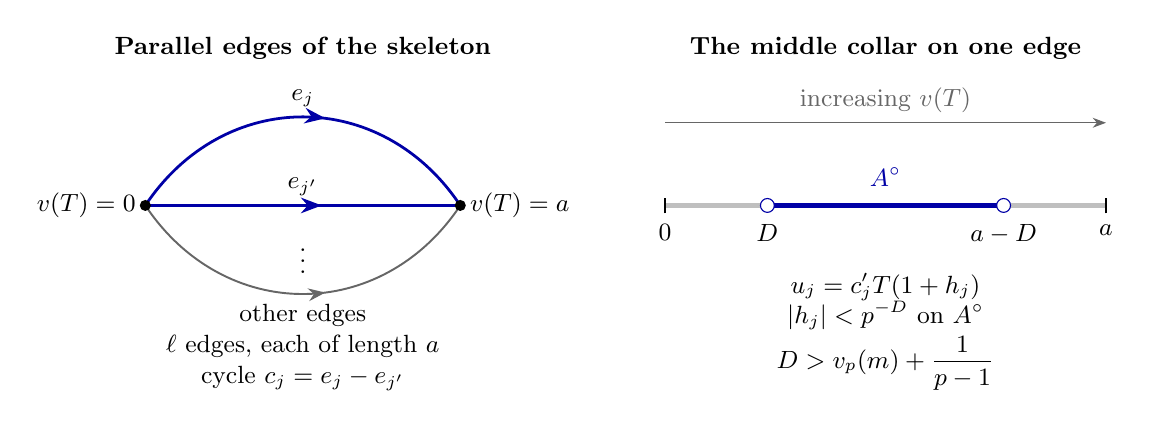
\begin{tikzpicture}[
  x=1cm,y=1cm,
  every node/.style={font=\small},
  directed/.style={postaction={decorate},decoration={markings,
    mark=at position 0.56 with {\arrow{Stealth}}}},
  selected/.style={blue!65!black,line width=1pt,directed},
  ordinary/.style={black!60,line width=.7pt,directed}
]
  \node[font=\small\bfseries] at (2,2.0) {Parallel edges of the skeleton};
  \draw[selected] (0,0) .. controls (1,1.5) and (3,1.5) .. (4,0);
  \draw[selected] (0,0) -- (4,0);
  \draw[ordinary] (0,0) .. controls (1,-1.5) and (3,-1.5) .. (4,0);
  \fill (0,0) circle (2pt);
  \fill (4,0) circle (2pt);
  \node[above] at (2,1.13) {$e_j$};
  \node[above] at (2,0) {$e_{j'}$};
  \node at (2,-.60) {$\vdots$};
  \node[below] at (2,-1.13) {other edges};
  \node[left,align=right] at (0,0) {$v(T)=0$};
  \node[right,align=left] at (4,0) {$v(T)=a$};
  \node[align=center] at (2,-2.00)
    {$\ell$ edges, each of length $a$\\cycle $c_j=e_j-e_{j'}$};

  \node[font=\small\bfseries] at (9.4,2.0) {The middle collar on one edge};
  \draw[-{Stealth},black!60] (6.6,1.05) -- (12.2,1.05)
    node[midway,above] {increasing $v(T)$};
  \draw[black!25,line width=2pt] (6.6,0) -- (12.2,0);
  \draw[blue!65!black,line width=2pt] (7.9,0) -- (10.9,0);
  \draw (6.6,-.10) -- (6.6,.10);
  \draw (12.2,-.10) -- (12.2,.10);
  \draw[blue!65!black,fill=white] (7.9,0) circle (2.5pt);
  \draw[blue!65!black,fill=white] (10.9,0) circle (2.5pt);
  \node[below] at (6.6,-.12) {$0$};
  \node[below] at (7.9,-.12) {$D$};
  \node[below] at (10.9,-.12) {$a-D$};
  \node[below] at (12.2,-.12) {$a$};
  \node[above,text=blue!65!black] at (9.4,.12) {$A^\circ$};
  \node[align=center] at (9.4,-1.22)
    {$u_j=c_j'T(1+h_j)$\\$|h_j|<p^{-D}$ on $A^\circ$};
  \node at (9.4,-2.00) {$D>v_p(m)+\dfrac{1}{p-1}$};
\end{tikzpicture}
\caption{The construction in Proposition~\ref{prop:arbitrary-roots},
shown schematically. All edges are oriented by increasing $v(T)$;
the cycle $e_j-e_{j'}$ gives a character unit $u_j$ of slope one
on the annulus corresponding to $e_j$. Division by $m$ on the Jacobian
supplies a root of $u_j$ on the whole inverse annulus. Trimming its
skeletal interval to $D<v(T)<a-D$ makes $h_j$ small enough for
$1+h_j$ to have an $m$-th root, and hence gives a root of $T$.}
\label{fig:parallel-edges}
\end{figure}


On every closed subannulus this estimate has a
strict uniform margin. The logarithm and exponential therefore
converge locally uniformly and
\[
 b_j=\exp\bigl(m^{-1}\log(1+h_j)\bigr)
\]
is analytic there, with $b_j^m=1+h_j$. Indeed, since
$D>1/(p-1)$, the logarithm satisfies
$|\log(1+h_j)|\le |h_j|$, and the valuation of the exponent is
greater than $D-v_p(m)>1/(p-1)$.

For all $\ell$ annuli at once, form the same algebraic finite \'etale cover
\[
 Z'=Z\times_{i,J,[m]}J\longrightarrow Z.
\]
It is finite \'etale for every positive integer $m$, since the ground
field has characteristic zero. Lemma~\ref{lem:division-roots} applied
to $a=\widehat i_j$ gives an analytic $m$-th root of $u_j$ on the
whole inverse image of $A_j$. Dividing it by $b_j$ and an $m$-th root
of $c_j'$ gives an analytic $m$-th root of $T$ above the middle
collar. The annuli $A_j$ are disjoint, so this gives a root on its
entire inverse image in $Z'$. Choose any connected component $Q$ of
$Z'$. Its map to $Z$ is finite \'etale and surjective, so it is a smooth
proper connected curve with the required property. Its composite
with $Z\to\mathbb P^1$ has only ramification indices $1$ or $\ell$.
All algebraic maps used to define $Q$ are over $\overline{k}$; the
analytic roots and torus lifts are only required over $\Omega$.
\end{proof}

\section{From collar roots to the completed universal tower}
\label{sec:realization}

The first stage, Proposition~\ref{prop:first-stage}, places the field
$L_\ell$ inside $H$.  We now use the auxiliary covers from
Proposition~\ref{prop:arbitrary-roots} to realize every finite Galois
extension of $K_0$ in that same completion.  The covers used to create
the collars may be branched; their horizontal ramification indices
divide $\ell$, so the first stage is sufficient to accommodate them.

\begin{proof}[Proof of Theorem~\ref{thm:completion}]
Let $F/K_0$ be any finite Galois extension inside $K^{\mathrm{sep}}$,
and let $C\to X_{\bar k}$ be its smooth proper curve cover.  Its branch
set $B$ is finite.  If $B$ is empty, then $F\subset\widetilde K\subset
H$ by definition of the universal étale field.  Suppose henceforth
that $B$ is nonempty.

For each $b\in B$, choose a rational local parameter $t_b$ at $b$ and
disjoint disks $B_b$ as in Lemma~\ref{lem:local-normal-form}; these
disks avoid $\xi$.  Let $m_b$ be the least common multiple of the
ramification indices of $C$ at the points above $b$.  Choose
$\beta_b\in\bar k^\times$ whose absolute value is smaller than the
radius of $B_b$ in the coordinate $t_b$.

Apply Proposition~\ref{prop:arbitrary-roots} with $m=m_b$.  In its
notation choose a positive integer $D_b>v_p(m_b)+1/(p-1)$ and
$\alpha_b\in\bar k^\times$ with
$a_b=-\log_p|\alpha_b|>2D_b$.  It gives a smooth proper connected
curve cover of the $T$-line whose horizontal indices divide $\ell$
and on whose full inverse image of
\[
                     D_b<-\log_p|T|<a_b-D_b
\]
the coordinate $T$ has an analytic $m_b$-th root.  Pull this cover back
by the nonconstant morphism $X_{\bar k}\to\mathbb P^1_{\bar k}$
given by $T=t_b/\beta_b$, and take a normalized connected component.
Denote the resulting cover by $W_b\to X_{\bar k}$.

Lemma~\ref{lem:horizontal-closure} shows that its horizontal indices
still divide $\ell$.  Roots pull back to every point of the normalized
component, so $t_b$ has an analytic $m_b$-th root on the entire inverse
image in $W_{b,\Omega}^{\mathrm{an}}$ of the collar
\[
 |\beta_b|p^{-(a_b-D_b)}<|t_b|<|\beta_b|p^{-D_b}
\]
inside $B_b$.  Here we multiplied the pulled-back root of $T$ by an
$m_b$-th root of $\beta_b$ in $\Omega$.

Embed the finitely many function fields $\bar k(W_b)$ into the fixed
$K^{\mathrm{sep}}$ over $K_0$ and form their compositum.  Let
$W\to X_{\bar k}$ be the associated smooth proper connected curve.
It dominates every $W_b$; its horizontal indices divide $\ell$ by
Lemma~\ref{lem:horizontal-closure}.  All collar roots therefore pull
back to the full inverse images in $W_\Omega^{\mathrm{an}}$.

Proposition~\ref{prop:patching}, with $Y=W_\Omega$, produces a
connected finite étale cover $V_\Omega\to W_\Omega$ and an analytic
map from its exterior region to $C_\Omega^{\mathrm{an}}$ over
$X_\Omega^{\mathrm{an}}$.  Since $W$ is proper over the algebraically
closed field $\bar k$, invariance of finite étale covers under the
algebraically closed extension $\bar k\subset\Omega$ \cite{SGA1}
gives a connected finite étale cover $V\to W$ and an isomorphism
\[
                  V\times_{\bar k}\Omega\simeq V_\Omega
                  \quad\text{over }W_\Omega.
\]
No descent assertion is needed for the exterior analytic map.

Although no such bound was imposed on $C\to X_{\bar k}$, the composite
$V\to X_{\bar k}$ still has horizontal indices dividing $\ell$.
By Lemma~\ref{lem:horizontal-closure}, its function
field embeds over $K_0$ in $L_\ell$.  This embedding can, if desired,
be chosen to extend the already chosen embedding of $\bar k(W)$:
extend that embedding to $\bar k(V)$ inside $K^{\mathrm{sep}}$ and
then take its Galois closure, which still has indices dividing $\ell$.
Proposition~\ref{prop:first-stage} places its image in $H$.

Lemma~\ref{lem:point-transfer} now gives a $K_0$-embedding
$F=\bar k(C)\hookrightarrow H\subset E$.  Because $F/K_0$ is
normal, this embedding has image the chosen subfield $F$ of $E$.
Indeed a primitive element of $F$ is sent to a root of its minimal
polynomial, all of whose roots already belong to $F$; the same holds
for every element.  The image, having degree $[F:K_0]$, is therefore
$F$ itself.  Consequently $F\subset H$.

Every element of $K^{\mathrm{sep}}$ lies in a finite Galois extension
of $K_0$ inside $K^{\mathrm{sep}}$: this is an algebraic closure of
the characteristic-zero field $K_0$.  Taking the union over those
extensions proves $K^{\mathrm{sep}}\subset H$ inside $E$.
\end{proof}

\section{From completion to point sections}\label{sec:sections}

We now use Theorem~\ref{thm:completion} to compare decomposition groups.
The comparison lifts any section localized at a rank-one valuation to a
birational section.  Koenigsmann's theorem then places the same section at
a rational point, and the two valuations give a contradiction.  The
remaining valuations are horizontal refinements, where the localization
theorem of Pop--Stix already identifies the section.

\begin{corollary}\label{cor:decomposition}
Let $k/\mathbb Q_p$ be finite and let $X/k$ be a smooth proper
geometrically connected curve of genus at least two.  Put $K=k(X)$ and
let $\widetilde K\subset K^{\mathrm{sep}}$ be the extension corresponding
to the full arithmetic \'etale fundamental group of $X$.  Let $w$ be a
real-valued rank-one valuation of $K$ extending the $p$-adic valuation,
normalized by $w(p)=1$, and fix a prolongation $w^{\mathrm{sep}}$ to
$K^{\mathrm{sep}}$.  Restriction induces an isomorphism of profinite
groups
\[
 D_{w^{\mathrm{sep}}}(K^{\mathrm{sep}}/K)
 \xrightarrow{\ \sim\ }
 D_{\widetilde w}(\widetilde K/K),
 \qquad \widetilde w=w^{\mathrm{sep}}|_{\widetilde K}.
\]
\end{corollary}

\begin{proof}
Restriction is surjective.  Indeed, lift an automorphism stabilizing
$\widetilde w$ to an automorphism of $K^{\mathrm{sep}}/K$.  Its translate
of $w^{\mathrm{sep}}$ is another prolongation of $\widetilde w$.
Transitivity of $\operatorname{Gal}(K^{\mathrm{sep}}/\widetilde K)$ on
these prolongations allows us to adjust the lift so that it stabilizes
$w^{\mathrm{sep}}$.  The transitivity statement for an infinite normal
extension follows from its finite-level version by compactness.

An automorphism stabilizing a rank-one valuation preserves its normalized
absolute value.  To see why normalization matters, any two
order-preserving embeddings of the value group into $\mathbb R$ differ
by a positive scale; the value on $p$ fixes that scale.  Such an
automorphism therefore extends as an isometry to
$E=\widehat{K^{\mathrm{sep}}}$.  If its restriction to $\widetilde K$ is
the identity, it fixes $H=\widehat{\widetilde K}\subset E$ pointwise.
Theorem~\ref{thm:completion} gives $K^{\mathrm{sep}}\subset H$, so the
automorphism is the identity.

Both decomposition groups are closed subgroups of their Galois groups.
For example, stabilization of a valuation ring is the intersection,
over its algebraic elements, of conditions on finite Galois orbits, each
of which is clopen.  Restriction is consequently a continuous bijection
between compact Hausdorff groups, and its inverse is continuous.
\end{proof}

\begin{lemma}\label{lem:no-rank-one-section}
With $k$, $X$, $K$, and $\widetilde K$ as in
Corollary~\ref{cor:decomposition}, let $w$ be any rank-one valuation of
$K$ extending the $p$-adic valuation and let $\widetilde w$ be any
prolongation to $\widetilde K$.  The projection
\[
 D_{\widetilde w}(\widetilde K/K)\longrightarrow G_k
\]
has no continuous group-homomorphic section.
\end{lemma}

\begin{proof}
Normalize $w(p)=1$ and prolong the valuation to $K^{\mathrm{sep}}$.
Suppose that a section exists.  Corollary~\ref{cor:decomposition} lifts
it to a continuous section
\[
 \widehat s:G_k\longrightarrow G_K
       =\operatorname{Gal}(K^{\mathrm{sep}}/K)
\]
whose image stabilizes this prolongation.  The birational section
theorem of Koenigsmann places the entire image of $\widehat s$ also in
the decomposition group of a prolongation of $\operatorname{ord}_a$ for
some $a\in X(k)$ \cite[preprint version, Proposition~2.4(2), Definition~1.4, and
Observation~1.3]{Koenigsmann}.  Here $\operatorname{ord}_a$ is the
closed-point valuation of $K$, trivial on $k$.

Write $\Sigma=\widehat s(G_k)$ and $M=(K^{\mathrm{sep}})^\Sigma$.
The subgroup $\Sigma$ is compact and hence closed, so
$G_M=\Sigma$.  Let $v_1$ and $v_2$ be the restrictions to $M$ of the two
selected prolongations.  Each is henselian: its absolute Galois group
stabilizes a prolongation, and the transitive action on all
prolongations therefore has a single point.  Both valuations are
nontrivial and have rank one.  Indeed, value groups in an algebraic
valued extension differ by a torsion quotient, which preserves their
convex-subgroup chains.  Moreover,
\[
 v_1(p)=1,\qquad v_2|_{k^\times}=0,
\]
so these valuations are inequivalent.  The resulting contradiction is
an instance of the classical uniqueness principle for henselian
valuations associated with F.~K.~Schmidt \cite{SchmidtValuations}.
We give explicitly the two-valuation approximation needed here.

Choose a nonsquare $d\in k^\times$.  It remains a nonsquare in $M$:
otherwise $G_M=\Sigma$ would fix a square root of $d$ in $\bar k$,
contrary to the surjection $\Sigma\to G_k$.  Let $t\in K$ be a
uniformizer at $a$.  Choose a positive integer $N$ with $N>v_1(t)$,
and put $z=p^N/t$.  Then
\[
 v_1(z)>0,\qquad v_2(z)=-v_2(t)<0.
\]
For positive integers $r$, set
\[
 q_r=d+(1-d)\frac{z^r}{1+z^r}.
\]
The denominator is nonzero because $v_1(z^r)>0$.  At the first
valuation $q_r$ tends to $d$, and at the second it tends to $1$.
More precisely,
\[
 v_1(q_r/d-1)
   =v_1((1-d)/d)+r v_1(z)\longrightarrow+\infty,
\]
whereas
\[
 v_2(q_r-1)
   =v_2(d-1)-r v_2(z)\longrightarrow+\infty.
\]
For sufficiently large $r$, Hensel's lemma applied at $1$ gives a
square root of $q_r/d$ using $v_1$, and a square root of $q_r$ using
$v_2$.  The sufficient inequalities are
\[
 v_1(q_r/d-1)>2v_1(2),\qquad
 v_2(q_r-1)>2v_2(2).
\]
Their quotient makes $d$ a square in $M$, a contradiction.  This
argument includes $p=2$ and arbitrary nondiscrete rank-one value groups.
\end{proof}

\begin{proof}[Proof of the surjectivity in Theorem~\ref{thm:section}]
Let $s:G_k\to\Pi_X$ be a continuous group-homomorphic section.
By the valuative localization theorem of Pop--Stix
\cite[preprint version, Theorem~26]{PopStix}, there is a valuation $w$ of $K$ extending
the $p$-adic valuation, together with a prolongation $\widetilde w$ to
$\widetilde K$, such that
\[
 s(G_k)\subseteq D_{\widetilde w}(\widetilde K/K).
\]
We classify the possibilities for $w$.

The valuation transcendence inequality gives
\[
 \operatorname{ratrank}(\Gamma_w/\Gamma_k)\leq 1.
\]
Since $\Gamma_k$ has rational rank one and ordered rank is at most
rational rank, $w$ has rank at most two.  Rank one is excluded by
Lemma~\ref{lem:no-rank-one-section}.  If $w$ has rank two, let $u$ be
its rank-one coarsening.  The nonzero proper convex subgroup of the
rank-two value group has a unique extension to the value group of
$\widetilde w$: it consists of those values some positive multiple of
which lies in the original subgroup.  This follows because an algebraic
valued extension has torsion quotient of value groups.  Every
automorphism stabilizing $\widetilde w$ preserves this subgroup, so
$s(G_k)$ stabilizes the resulting prolongation of $u$.  If $u$
is nontrivial on $k$, it can be normalized to extend the $p$-adic
valuation and is excluded by the same lemma.

It remains that $u$ is trivial on $k$.  Properness gives it a center
on $X$.  This center cannot be generic because $u$ is nontrivial, so
it is a closed point $a$.  The valuation ring of $u$ dominates the
discrete valuation ring $\mathcal O_{X,a}$.  Every element of $K^\times$
is a power of a uniformizer times a unit of this local ring; hence
$u$ is equivalent to $\operatorname{ord}_a$.  Its residue field is the
finite extension $k(a)/k$.  The second valuation in the composition
$w$ is the unique prolongation of the $p$-adic valuation to $k(a)$.
Thus $w$ is of type $2h$.

The chosen horizontal prolongation to $K\bar k$ selects a geometric
point above $a$.  Its stabilizer acts on constants through
$G_{k(a)}\subseteq G_k$, with the embedding determined by that point.
Since $s(G_k)$ projects onto $G_k$, necessarily $k(a)=k$.
For the full \'etale tower the horizontal inertia is trivial, and the
horizontal decomposition group is the point section at $a$.
Equivalently, the type-$2h$ conclusion of
\cite[preprint version, Section~6.1]{PopStix} gives $s=s_a$ after the corresponding
geometric choice of base point.  This proves surjectivity.

Notice that a type-$2h$ valuation can lie over a non-rational closed
point.  Rationality here follows from the surjection to $G_k$; no
unrestricted equivalence between ``not type $2h$'' and ``not originating
from a rational point'' is used.
\end{proof}

\begin{proof}[Proof of the injectivity in Theorem~\ref{thm:section}]
Suppose $a,b\in X(k)$ have the same section class modulo the full
geometric fundamental group.  Let $J$ be the Jacobian of $X$, and use
$a$ as base point for the Abel--Jacobi map
\[
 i_a:X\longrightarrow J,\qquad x\longmapsto [x-a].
\]
Their induced sections on $J$ are again geometrically conjugate.
For every positive integer $n$, multiplication
$[n]:J\to J$ is a finite \'etale torsor under $J[n]$, also when
$p\mid n$ since $k$ has characteristic zero.  Conjugate sections give
isomorphic $G_k$-actions on its geometric fiber, so the existence of a
fixed point is unchanged by conjugation.  The section at $i_a(a)=0$
has the fixed lift $0$.  Therefore the fiber over $i_a(b)$ has a
$G_k$-fixed point, which is a $k$-rational point of that fiber.  Thus
\[
 i_a(b)\in\bigcap_{n\geq1}nJ(k).
\]
This is also the usual Kummer argument: the class of the multiplication
torsor pulled back along a section is unchanged by geometric conjugation.

The compact $p$-adic analytic group $J(k)$ has an open subgroup
$U\cong\mathbb Z_p^{g(X)[k:\mathbb Q_p]}$ by the local logarithm.  If
$q=[J(k):U]$, then $qJ(k)\subseteq U$.  For each $r\geq0$, take
$n=qp^r$ in the displayed intersection.  Any element of that intersection
can then be written as $p^r(qy)$ with $y\in J(k)$, and hence belongs
to $p^rU$.  As $U$ is a finite free $\mathbb Z_p$-module,
\[
 \bigcap_{r\geq0}p^rU=0,
\]
and hence $i_a(b)=0$.  If $a\ne b$, the linear equivalence of the
degree-one divisors $a$ and $b$ would give a degree-one morphism
$X\to\mathbb P^1$, forcing genus zero.  Hence $a=b$, as required.
\end{proof}

\section{Global consequences via finite descent}\label{sec:global-sections}

We now combine the local theorem with established descent and
finite-support results. First we identify the adelic tuples obtained
from global sections. We then
give a criterion that makes these sections geometric and apply it to
abelian targets and modular curves. Finally, we describe further
restrictions on the localization tuples without assuming that criterion.
In this section $K$ is a number field. For a
field $F$ of characteristic zero and a smooth proper geometrically
connected curve $D/F$, write $\operatorname{Sec}(D/F)$ for the
conjugacy classes of continuous splittings of
\[
 1\longrightarrow\pi_1(D_{\bar F})\longrightarrow\pi_1(D)
   \longrightarrow G_F\longrightarrow1,
 \qquad G_F=\operatorname{Gal}(\bar F/F),
\]
where conjugation is by the full geometric \'etale fundamental group.
For a smooth proper geometrically connected curve $C/K$ of genus at
least two, the global section conjecture asserts that the point map
\[
 \kappa_C:C(K)\longrightarrow\operatorname{Sec}(C/K)
\]
is bijective. Thus the section classes considered here are the full
arithmetic \'etale classes, without a birational lifting assumption.

\subsection{Localization and descent}\label{subsec:global-localization}

For a proper $K$-scheme $V$, use the modified adelic set
\[
 V(\mathbb A_K)_\bullet
 =\prod_{v\nmid\infty}V(K_v)
  \times\prod_{v\ \mathrm{real}}\pi_0\bigl(V(K_v)\bigr),
\]
where $\pi_0$ denotes the set of connected components. Complex places
are omitted, as in the corrected convention of Stoll's erratum
\cite[Section~1]{StollFiniteDescentErrata}. For geometrically connected
$C$ the complex component factors in the earlier convention are
singletons, but their omission matters for geometrically disconnected torsors.
A point of $C(\mathbb A_K)_\bullet$ survives a torsor $Y\to C$ under a
finite $K$-group scheme $G$ if it lifts to
$Y^\xi(\mathbb A_K)_\bullet$ for some twist $Y^\xi$, where
$\xi\in H^1(K,G)$.
Write $C(\mathbb A_K)_\bullet^{\mathrm{f\text{-}cov}}$ for the points
surviving every such torsor, and
$C(\mathbb A_K)_\bullet^{\mathrm{f\text{-}ab}}$ for those surviving
every such torsor with $G$ abelian
\cite[Definitions~5.2 and~5.4]{StollFiniteDescent}. We identify $C(K)$ with its
diagonal image. The definitions give
\begin{equation}\label{eq:descent-inclusions}
 C(K)\subseteq C(\mathbb A_K)_\bullet^{\mathrm{f\text{-}cov}}
 \subseteq C(\mathbb A_K)_\bullet^{\mathrm{f\text{-}ab}}.
\end{equation}

The local section theorems define a localization map for every such
curve, without any descent equality hypothesis.
Let $s\in\operatorname{Sec}(C/K)$. At every finite place $v$, its
localization is the section of a unique point $P_v\in C(K_v)$ by
Theorem~\ref{thm:section}. At a real place the section map
\[
 \pi_0\bigl(C(K_v)\bigr)\longrightarrow\operatorname{Sec}(C/K_v)
\]
is bijective by the real section theorem; the genus-at-least-two case
is included in the theorem of Bresciani--Vistoli
\cite[Introduction, Theorem]{BrescianiVistoliReal}. At a complex place
the local Galois group is trivial and the local condition is automatic.
Thus $s$ is a Selmer section: it comes from a local point at every
place. Properness makes these localizations a modified adelic point
$x(s)\in C(\mathbb A_K)_\bullet$. We obtain the canonical map
\[
 \operatorname{loc}:\operatorname{Sec}(C/K)
 \longrightarrow C(\mathbb A_K)_\bullet,
 \qquad s\longmapsto x(s).
\]

\begin{proposition}[The localization image]\label{prop:localization-image}
Let $C/K$ be a smooth proper geometrically connected curve of genus at
least two over a number field. Then
\begin{equation}\label{eq:localization-image}
 \operatorname{loc}\bigl(\operatorname{Sec}(C/K)\bigr)
 =C(\mathbb A_K)_\bullet^{\mathrm{f\text{-}cov}}.
\end{equation}
\end{proposition}

\begin{proof}
Let $s\in\operatorname{Sec}(C/K)$.
Choose a representative point of the determined component at each
real place, and any point at each complex place. Harari--Stix's
Theorem~2.1, with $U=1$ and the omitted set of places $S=\varnothing$,
shows that these localizations survive every torsor under a finite
$K$-group scheme; their Remark~2.2(1) identifies this as finite-cover
descent \cite[preprint version, Theorem~2.1 and Remark~2.2(1)]{HarariStixFiniteDescent}.
Consequently
\[
 x(s)\in C(\mathbb A_K)_\bullet^{\mathrm{f\text{-}cov}}.
\]

Conversely, let $x$ belong to the
finite-cover locus and, by properness, choose an ordinary adelic
representative $P=(P_v)\in C(\mathbb A_K)$. Stoll's cohomological description after
Definition~5.2, together with Definition~5.4, identifies survival with
diagonal global $H^1(K,G)$-membership of the local evaluations for
every torsor under a finite $K$-group scheme $G$
\cite{StollFiniteDescent}. These evaluations factor through the real
components, and complex places impose no lifting condition, in the
corrected convention already used above. Thus every such $P$ satisfies
the ordinary finite-torsor condition. Harari--Stix's Theorem~2.1 with
$U=1$ and $S=\varnothing$, using implication (i)$\Rightarrow$(iii),
gives a global section whose restrictions are the point sections of
$P_v$, up to conjugation by the full geometric fundamental group
\cite[preprint version, Theorem~2.1 and Remark~2.2(1)]{HarariStixFiniteDescent}.
The finite-point and real-component uniqueness used above identify its
localization with $x$, proving~\eqref{eq:localization-image}.
\end{proof}

\subsection{Criteria for point sections}\label{subsec:global-criteria}

Proposition~\ref{prop:localization-image} determines which adelic tuples
come from sections. To recover rational points from the sections
themselves, we also need the finite-support theorem of Stix.

\begin{theorem}[Finite-cover descent criterion]\label{thm:global-descent}
Let $C/K$ be a smooth proper geometrically connected curve of genus at
least two over a number field. If
\begin{equation}\label{eq:finite-cover-equality}
 C(\mathbb A_K)_\bullet^{\mathrm{f\text{-}cov}}=C(K),
\end{equation}
then $\kappa_C:C(K)\to\operatorname{Sec}(C/K)$ is bijective.
\end{theorem}

\begin{proof}
Let $s\in\operatorname{Sec}(C/K)$. By
Proposition~\ref{prop:localization-image} and
\eqref{eq:finite-cover-equality}, there is $a\in C(K)$ such that
$x(s)$ is the diagonal localization of $a$, hence equals the
localization of the point section $s_a$.

At every finite place the point determined by $s$ is therefore $a$.
At each real place choose $a$ itself in the determined component,
and choose $a$ also at each complex place. The resulting ordinary
adelic representative of the localization tuple is supported on
$\{a\}$. Thus the support $Z(s)$ in Stix's terminology, the
Zariski-closed support of this tuple, is finite over $K$.
Since $C$ is proper of genus at least two, it is hyperbolic and has no
cuspidal sections. Stix's finite-support result therefore makes $s$
a point section \cite[arXiv version, Section~3 and Corollary~5]{StixFiniteSupport}.
Finally, if two points give the same global section, their sections
agree after restriction to any one finite completion. Injectivity in
Theorem~\ref{thm:section} then identifies the two points. This proves
injectivity and also identifies the point giving $s$ with $a$.
\end{proof}

The equality in~\eqref{eq:finite-cover-equality} is supplied by several
published criteria. For an abelian variety $A/K$, let
\[
 \operatorname{Sha}(A/K)
 =\ker\left(H^1(K,A)\longrightarrow\prod_v H^1(K_v,A)\right),
\]
and write $\operatorname{Sha}(A/K)_{\mathrm{div}}$ for its maximal
divisible subgroup.

\begin{corollary}[Abelian targets]\label{cor:global-abelian-target}
Let $C/K$ be a smooth proper geometrically connected curve of genus at
least two over a number field. The map $\kappa_C$ is bijective if either
of the following conditions holds:
\begin{enumerate}[label=\textnormal{(\roman*)}]
\item there is a nonconstant $K$-morphism $C\to A$ to an abelian
variety with $A(K)$ finite and $\operatorname{Sha}(A/K)_{\mathrm{div}}=0$;
\item the Jacobian $J$ of $C$ has $J(K)$ finite and
$\operatorname{Sha}(J/K)_{\mathrm{div}}=0$.
\end{enumerate}
\end{corollary}

\begin{proof}
Stoll's Theorem~8.6 gives
$C(\mathbb A_K)_\bullet^{\mathrm{f\text{-}ab}}=C(K)$ under the first
condition, and his Corollary~8.1 gives the same equality under the
second, without requiring a $K$-rational base point on $C$
\cite{StollFiniteDescent}. The corrected covering arguments and the
repair of Proposition~8.5 used by Theorem~8.6 are in
\cite[Sections~2--3]{StollFiniteDescentErrata}; the stated equalities
are retained. The inclusions~\eqref{eq:descent-inclusions} now imply
\eqref{eq:finite-cover-equality}, so Theorem~\ref{thm:global-descent}
applies.
\end{proof}

For an elliptic curve $E/\mathbb Q$ and a prime $p$, put
\[
 s_p(E)=\operatorname{corank}_{\mathbb Z_p}
        \operatorname{Sel}_{p^\infty}(E/\mathbb Q),
\]
where the Selmer group uses the local Kummer conditions at every place.

\begin{corollary}[A Selmer-corank-zero elliptic target]\label{cor:global-selmer-target}
Let $C/\mathbb Q$ be a smooth proper geometrically connected curve of
genus at least two. Suppose that there is a nonconstant
$\mathbb Q$-morphism $C\to E$ to an elliptic curve and that $s_p(E)=0$
for at least one prime $p$. Then $\kappa_C$ is bijective.
\end{corollary}

\begin{proof}
\emergencystretch=2em
The corank-zero case of the companion Selmer converse
\cite[Theorem~1.1]{OpenAISelmerConverse2026} gives
$\operatorname{rank}_{\mathbb Z}E(\mathbb Q)=0$ and finiteness of the
entire group $\operatorname{Sha}(E/\mathbb Q)$. The Mordell--Weil
theorem therefore makes $E(\mathbb Q)$ finite, while finiteness of
$\operatorname{Sha}(E/\mathbb Q)$ makes its maximal divisible subgroup
zero. Corollary~\ref{cor:global-abelian-target}(i) applies.
\end{proof}

\begin{corollary}[Modular curves]\label{cor:global-modular-curves}
For every positive integer $N$ such that the smooth projective
geometrically connected curve $X_0(N)/\mathbb Q$ has genus at least two,
the map $\kappa_{X_0(N)}$ is bijective. The same assertion holds for the
smooth projective geometrically connected curve $X_1(N)/\mathbb Q$
whenever its genus is at least two.
\end{corollary}

\begin{proof}
Stoll's Corollary~8.8 gives
$C(\mathbb A_{\mathbb Q})_\bullet^{\mathrm{f\text{-}ab}}=C(\mathbb Q)$
for each of these projective modular curves of positive genus
\cite{StollFiniteDescent}, with the corrected conventions of
\cite{StollFiniteDescentErrata}. Apply~\eqref{eq:descent-inclusions}
and Theorem~\ref{thm:global-descent}.
\end{proof}

The general implication retains the finite-cover equality as a genuine
arithmetic hypothesis; local point-theoreticity alone does not supply
it. The elliptic-target specialization uses only Selmer corank zero over
$\mathbb Q$, while the modular-curve cases come directly from Stoll's
descent result and do not depend on that specialization.

\subsection{Further restrictions on localization}
\label{subsec:global-restrictions}

We return to an arbitrary smooth proper geometrically connected curve
$C/K$ of genus at least two over a number field, without
assuming~\eqref{eq:finite-cover-equality}. The localization image in
Proposition~\ref{prop:localization-image} satisfies additional descent
conditions and, under a restriction on $K$, has finite image at each
finite place.

Let $\rho:C(\mathbb A_K)\to C(\mathbb A_K)_\bullet$ be the natural
projection. Write $D_{\mathrm{lin}}(C)$ for the ordinary adelic descent
set: $P$ belongs to it if, for every $C$-torsor $T\to C$ under a linear
algebraic $K$-group $G$, it lifts to $T^\xi(\mathbb A_K)$ for some
global twist $\xi\in H^1(K,G)$. Harari--Stix's Theorem~4.1 sends the
finite-torsor condition established in
Proposition~\ref{prop:localization-image} to this linear descent
condition, while their Corollary~3.1, applied to the geometric
abelianization of the interpolating section, gives Brauer--Manin
membership
\cite[preprint version, Corollary~3.1 and Theorem~4.1]{HarariStixFiniteDescent}.
Consequently
\begin{equation}\label{eq:localization-obstructions}
 \rho^{-1}\!\left(\operatorname{loc}\bigl(\operatorname{Sec}(C/K)\bigr)\right)
 \subseteq D_{\mathrm{lin}}(C)\cap C(\mathbb A_K)^{\operatorname{Br}}.
\end{equation}
This applies to every ordinary adelic representative of a modified
localization tuple; the lifting condition uses ordinary adeles also
when $T$ is nonproper.

Finally, if $K$ contains no CM subfield, Betts--Stix's Theorem~A,
applied to the sections shown to be Selmer in
Section~\ref{subsec:global-localization}, gives
\[
 \#\operatorname{loc}_v\bigl(\operatorname{Sec}(C/K)\bigr)<\infty,
 \qquad
 \operatorname{loc}_v=\operatorname{pr}_v\circ\operatorname{loc},
\]
for every finite place $v$, with image in $C(K_v)$
\cite[arXiv version, Definition~1.1 and Theorem~A]{BettsStix}.
This asserts neither injectivity of localization nor finiteness of the
global section set, and supplies no effective or uniform bound.

\begingroup
\raggedright
\bibliographystyle{plain}
\bibliography{references}
\endgroup
\end{document}
